\documentclass{article}
\usepackage[margin=1in]{geometry}
\usepackage{amsmath,amsthm,amssymb}
\usepackage{bbm,enumerate,mathtools}
\usepackage{tikz,pgfplots}
\usepackage{chessboard}
\usepackage[hidelinks]{hyperref}
\usepackage{multicol} % Problem 35

\newenvironment{question}{\begin{trivlist}\item[\textbf{Question.}]}{\end{trivlist}}
\newenvironment{note}{\begin{trivlist}\item[\textbf{Note.}]}{\end{trivlist}}
\newenvironment{references}{\begin{trivlist}\item[\textbf{References.}]}{\end{trivlist}}
\newenvironment{related}{\begin{trivlist}\item[\textbf{Related.}]\end{trivlist}\begin{enumerate}}{\end{enumerate}}


\begin{document}
\rating{4}{3}
Consider ways to lay matchsticks (of unit length) on the $n \times m$ grid in
such a way as to form a maze.
\begin{figure}[ht!]
  \centering
  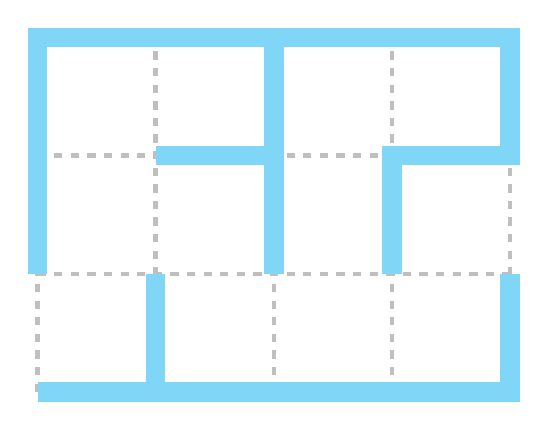
\begin{tikzpicture}[scale=1.5]
    \draw[ultra thick, gray!50, dashed] (0,0) grid (4,3);
    \draw[line width=0.25cm, cyan!50] (0,0)--(4,0)--(4,1);
    \draw[line width=0.25cm, cyan!50] (1,0)--(1,1);
    \draw[line width=0.25cm, cyan!50] (0,1)--(0,3)--(4,3)--(4,2)--(3,2)--(3,1);
    \draw[line width=0.25cm, cyan!50] (2,3)--(2,1);
    \draw[line width=0.25cm, cyan!50] (1,2)--(2,2);
  \end{tikzpicture}\hspace{0.5cm}
  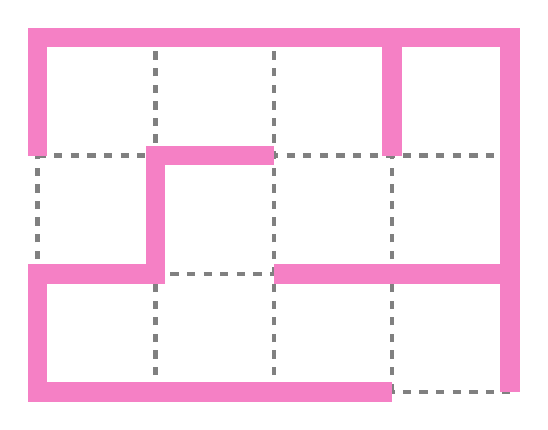
\begin{tikzpicture}[scale=1.5]
    \draw[ultra thick, gray, dashed] (0,0) grid (4,3);
    \draw[line width=0.25cm, magenta!50] (2,2)--(1,2)--(1,1)--(0,1)--(0,0)--(3,0);
    \draw[line width=0.25cm, magenta!50] (0,2)--(0,3)--(4,3)--(4,0);
    \draw[line width=0.25cm, magenta!50] (2,1)--(4,1);
    \draw[line width=0.25cm, magenta!50] (3,3)--(3,2);
    % \draw[line width=0.25cm, green!50] (4,0)--(4,1)--(2,1)--(2,0)--cycle;
  \end{tikzpicture}
  \caption{
    Two mazes on a $(5 \times 4)$-cell grid.
  }
\end{figure}
\begin{question}
  How many distinct mazes can be drawn on the grid?
\end{question}

\begin{related}
  \item What if every $1\times1$ cell must be reachable?
  \item What if there are no dead ends?
  \item What if there are to be identically $k$ dead ends?
  \item What if paths that loop are not allowed?
  \item What if the entrance and exit have prescribed positions?
  \item What if this is done on a hexagonal or triangular grid? On a torus?
  \item Is there a meaningful way to assign ``difficulty'' to a maze?
\end{related}
\begin{references}
  \item Problem 64.
\end{references}
\end{document}
